\section{Theorie}
\label{sec:theorie}

    In diesem Abschnitt werden die theoretischen Grundlagen der Ultraschalltechnik erläutert.

    Für die Ultraschalltechnik werden Frequenzen in einem Bereich von $\SI{20}{\kilo\hertz}$ bis $\SI{1}{\giga\hertz}$ verwendet,
    wobei dieser Bereich oberhalb des hörbaren Frequenzspektrums von $\SI{16}{\hertz}$ bis $\SI{20}{\kilo\hertz}$ liegt.
    Ultraschallwellen können,
    im Gegensatz zu Schallwellen aus dem hörbaren Spektrum,
    Gewebe durchdringen und werden deshalb in der Medizin oft verwendet.\\
    Die Schallwellen sind longitudinale Wellen,
    die sich aufgrund von Druckschwankungen in der Luft nach der Gleichung
    \begin{equation}
        p(x,t) = p_0 + v_0 Z \cos{\omega t - kx}
    \end{equation}
    ausbreiten.
    Ihre Phasengeschwindigkeit ist im Gegensatz zu elektromagnetischen Wellen materialabhängig.
    Die Größe $Z = c \cdot \rho$ bezeichnet die akustische Impedanz,
    welche abhängig von der Schallgeschwindigkeit $c$ im Medium und der Dichte $\rho$ des Mediums ist.\\
    \\
    Die Ausbreitung der Schallwelle verhält sich ebenfalls abhängig vom Medium.
    Es wird zwischen Flüssigkeiten und Festkörpern unterschieden.\\
    Die Schallgeschwindigkeit in Flüssigkeiten kann mit 
    \begin{equation}
        c_\text{Fl} = \sqrt{\frac{1}{\kappa \rho}}
        \label{eqn:schallgeschwindigkeit_flüssigkeit}
    \end{equation}
    beschrieben werden,
    wobei $\kappa$ die Kompressibilität darstellt.
    In Flüssigkeiten und Gasen ist die Schallwelle ausschließlich longitudinal.\\
    Die Schallgeschwindigkeit in Festkörpern kann mit 
    \begin{equation}
        c_\text{Fe} = \sqrt{\frac{E}{\rho}}
        \label{eqn:schallgeschwindigkeit_festkörper}
    \end{equation}
    beschrieben werden,
    wobei das Elastizitätsmodul $E$ gerade $\kappa^{-1}$ ist.
    In Festkörpern ist die Schallgeschwindigkeit richtungsabhängig und aufgrund von Schubspannungen breitet sie sich sowohl longitudinal,
    als auch transversal aus.

\subsection{Absorption von Ultraschallwellen}

    Wenn sich die Schallwelle im Medium ausbreitet,
    findet Absorption statt,
    was dazu führt,
    dass ein Teil der Energie verloren geht.
    Die Intensität mit dem Absorptionskoeffizienten $\alpha$
    \begin{equation}
        I(x) = I_0 \exp{(-\alpha x)}
    \end{equation}
    nimmt exponentiell mit der Strecke $x$ ab.
    Zur Abschwächung der Absorption in Luft wird ein Kontaktmittel zwischen Schallgeber und Material genutzt.
    Beim Auftreffen einer Schallwelle auf die Grenzfläche wird ein Teil der Welle reflektiert und ein Teil wird transmittiert.
    Für den Reflexionskoeffizienten $R$ ergibt sich
    \begin{equation}
        R = \Bigl(\frac{Z_1 - Z_2}{Z_1 + Z_2}\Bigr)^2 \ ,
        \label{eqn:reflexion}
    \end{equation}
    wobei sich das Verhältnis von einfallendem und reflektiertem Anteil durch die akustischen Impedanzen darstellen lässt.
    Für den Transmissionskoeffizienten gilt
    \begin{equation}
        T = 1 - R \ .
        \label{eqn:transmission}
    \end{equation}

\subsection{Erzeugung von Ultraschallwellen}

    Die hier verwendete Methode zur Erzeugung von Ultraschallwellen ist der reziproke piezo-elektrische Effekt.
    Dazu wird ein Piezokristall in ein elektrisches Wechselfeld gebracht,
    welches den Kristall zu Schwingungen anregt und Ultraschallwellen erzeugt,
    für den Fall,
    dass das elektrische Feld in eine der Polarrichtungen des Kristalls zeigt.
    Bei Resonanzfrequenzen können große Schwingungsamplituden entstehen,
    sodass große Schallenergiedichten verwendet werden können.\\
    Wenn der Piezokristall durch Schallwellen zum Schwingen angeregt wird, 
    kann er auch als Empfänger dienen.

\subsection{Messung mit Ultraschallwellen}

    Zur Messung mit Ultraschalltechnik werden Laufzeitmessungen durchgeführt,
    wobei ein kurzzeitiger Schallimpuls ausgesendet wird,
    dessen Laufzeit gemessen wird wenn er auf einen Empfänger trifft.\\
    \clearpage
    \begin{figure}
        \centering
        \begin{subfigure}{0.48\textwidth}
            \centering
            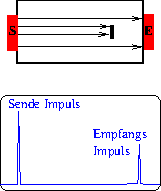
\includegraphics[width=0.75\textwidth]{content/img/Abb_1a.pdf}
            \caption{Das Durchschallungs-Verfahren zur Messung mit Ultraschallwellen.}
            \label{fig:durchschallung}
        \end{subfigure}
        \begin{subfigure}{0.48\textwidth}
            \centering
            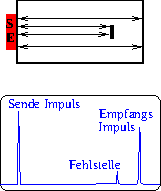
\includegraphics[width=0.75\textwidth]{content/img/Abb_1b.pdf}
            \caption{Das Impuls-Echo-Verfahren zur Messung mit Ultraschallwellen.}
            \label{fig:impuls_echo}
        \end{subfigure}
    \end{figure}

    Die Abbildungen \ref{fig:durchschallung} und \ref{fig:impuls_echo} zeigen zwei verschiedene Möglichkeiten,
    mithilfe von Ultraschalltechnik zu messen.\\
    Das Durchschallungs-Verfahren misst einen kurzzeitigen Schallimpuls,
    welcher an einem Sender erzeugt wird und durch eine Probe fliegt.
    Es wird die gemessene Intensität des Impulses untersucht,
    welche genau dann absinkt, 
    wenn die Schallwelle eine Fehlstelle passiert,
    wobei die genaue Position der Fehlstelle in der Probe mit diesem Verfahren nicht bestimmt werden kann.\\
    Das Impuls-Echo-Verfahren misst einen Schallimpuls,
    welcher an einer Grenzfläche reflektiert wird,
    sodass der Sender gleichzeitig auch als Empfänger dient.
    Bei diesem Verfahren kann die Position der Fehlstelle in der Probe mithilfe der Gleichung
    \begin{equation}
        s = \frac{1}{2} \cdot c t
        \label{eqn:position_fehlstelle}
    \end{equation}
    bestimmt werden,
    wobei $c$ die Schallgeschwindigkeit und $t$ die Laufzeit des Schallimpulses darstellt.
    Mithilfe eines A-/B-Scans oder TM-Scans können Laufzeitdiagramme erstellt werden.

